As previously mentioned, epigenetic marks are fundamental aspects of the cellular biological processes. 
Indeed, their state influences not only gene accession but also the regulation of gene expression.

Some relevant aspects are \glspl{hm} and \glspl{tf}, the first ones are related to transcriptional activation/inactivation, chromosome packaging, and \gls{dna} damage/repair.
While \glspl{tf}, also named as sequence-specific \gls{dna}-binding factor, are proteins that control the transcription of genetic information by binding specific sequences of \gls{dna}.

To investigate these epigenetic aspects nowadays is mainly used the Chromatin ImmunoPrecipitation sequencing (\textit{ChIP-seq}) technique \cite{Park2009}.
This technique allows to use antibodies for selected proteins or nucleosomes, which enriches for specific \gls{dna} sequences bounded to these proteins/nucleosomes.

\begin{figure}[H]
\centering
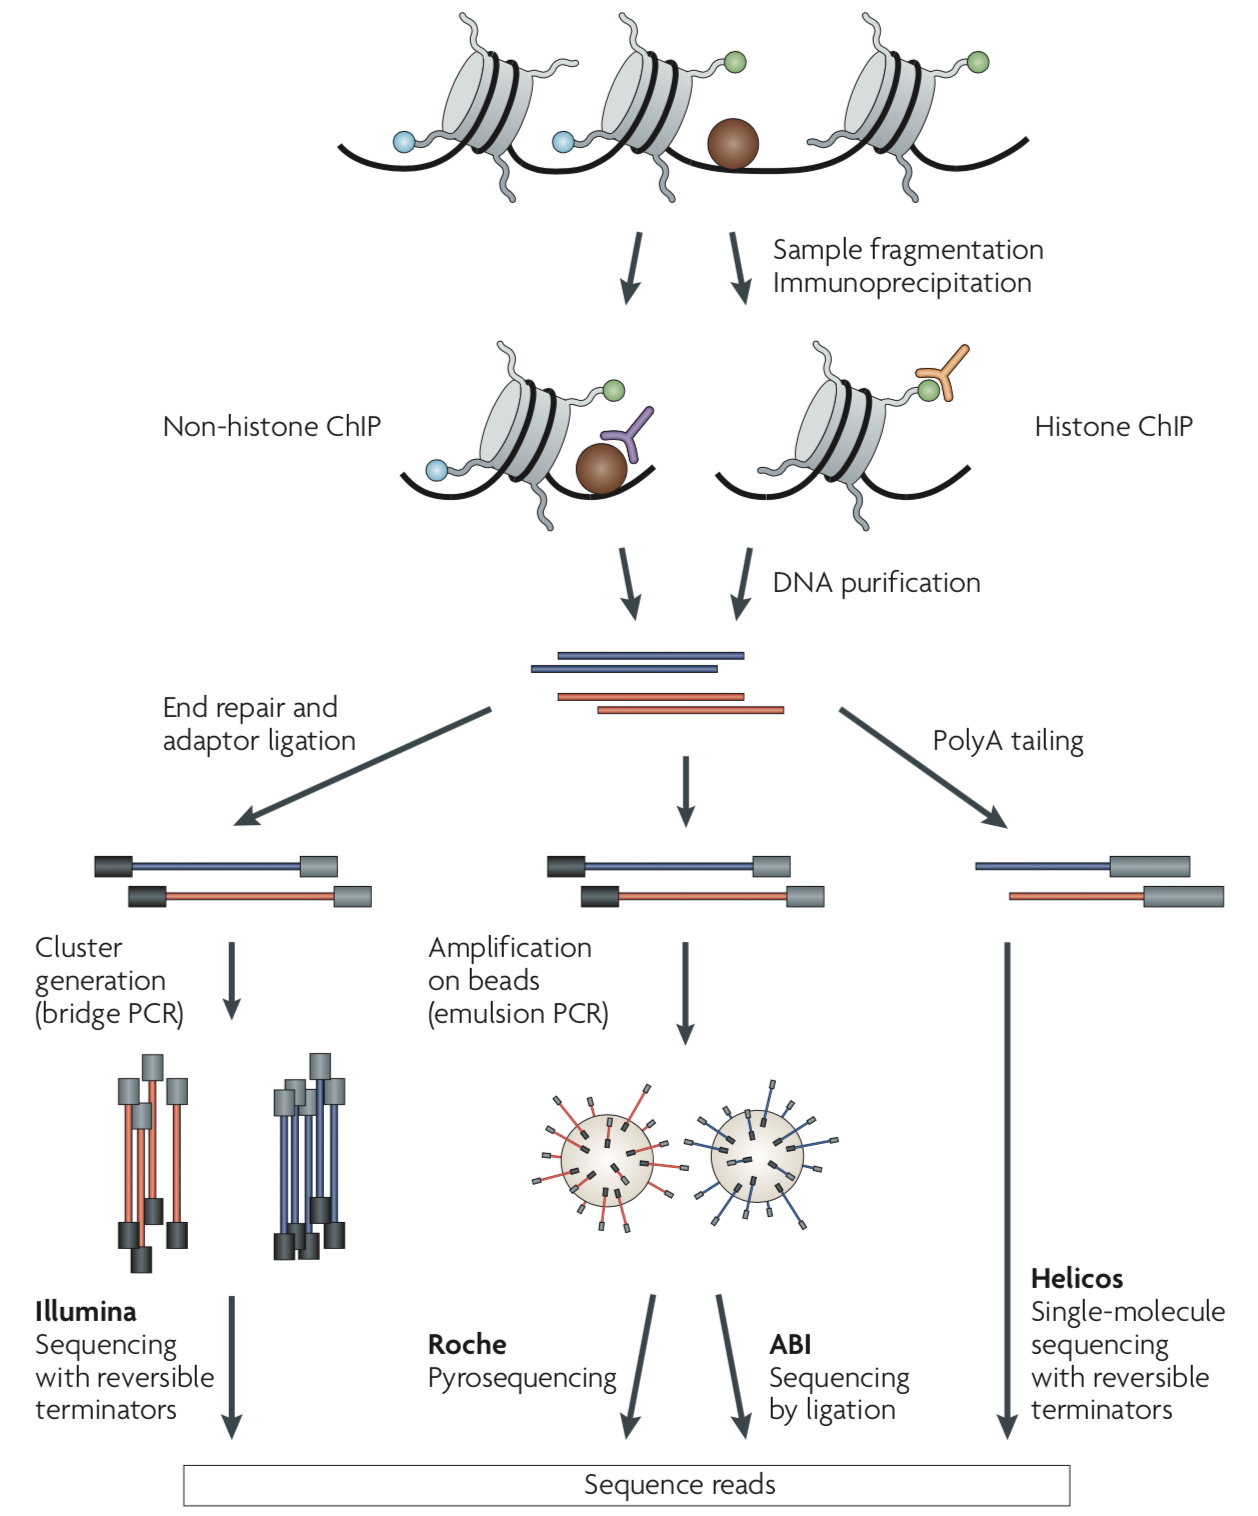
\includegraphics[width=8cm, keepaspectratio]{img/intro/chip.png}
\caption[ChIP-seq experiment]{Representation of a  ChIP-seq experiment. \cite{Park2009}}
\label{fig:chipseqexp}
\end{figure}

The library preparation consists into lock biological processes with formaldehyde and then cutting the chromatin into small fragments with sonication.
Afterwards, a specific antibody for the interested protein is used to immunoprecipitate the \gls{dna}-protein complex, in order to be purified and, after amplification, be sequenced.

When analyzing the data, it is relevant to distinguish between \gls{hm} and \gls{tf} ChIP because, even if the library preparation it's the same (it differs only for the antibody used, just because the proteins are different), the data analysis pipeline is different in methodologies used because of the different signal produced by them.
Indeed, after read mapping on a reference genome, reads need to be processed with methodologies for the protein-binding regions detection, that are typically called \textit{Peak callers}.
After the peak calling process it is possible to highlight that the \gls{tf} signals (peaks) are more narrowed respect to the ones detected for \gls{hm}, leading to develop different methodologies for investigating further aspects for each one of these \textit{ChIP-seq} signals.

\begin{figure}[H]
\centering
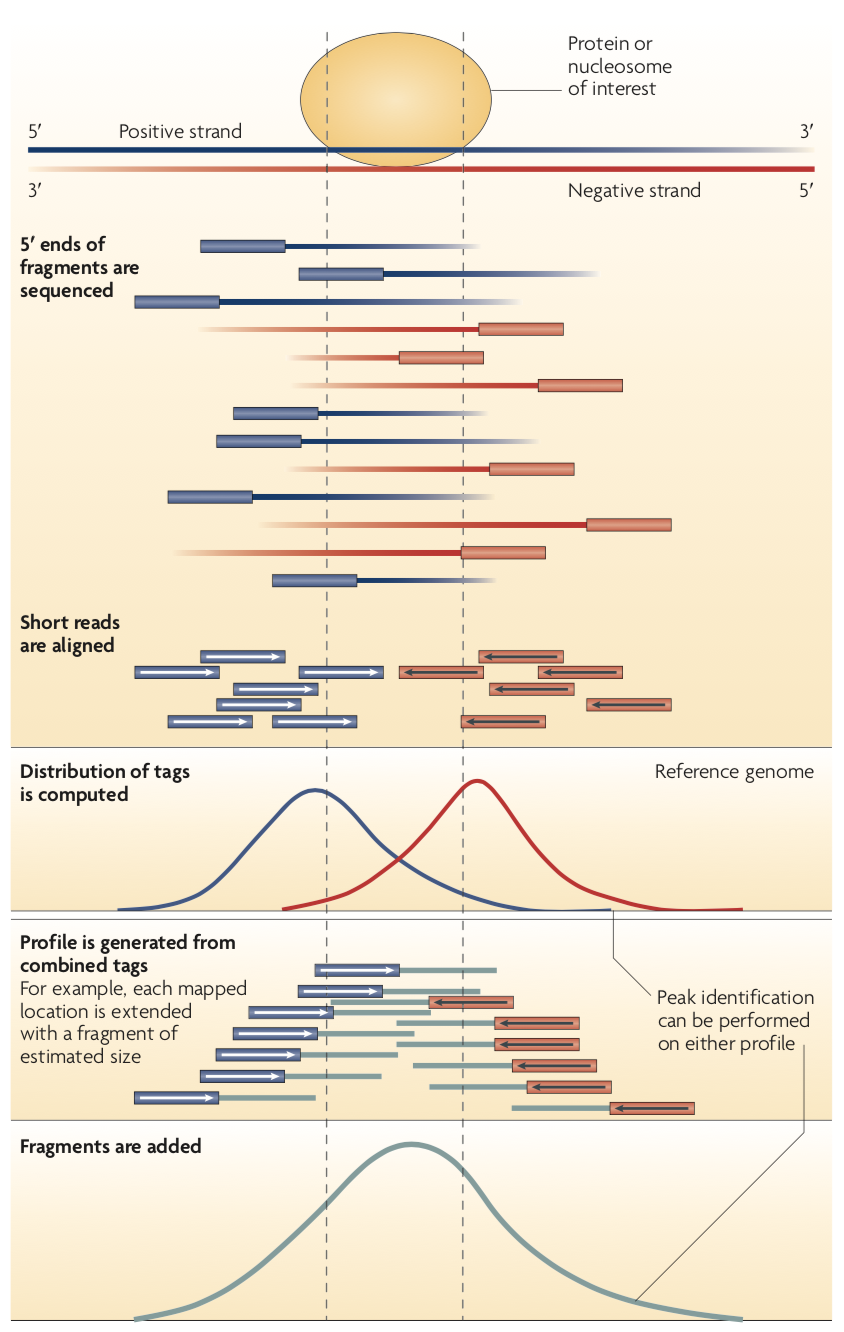
\includegraphics[width=8cm, keepaspectratio]{img/intro/peak_call.png}
\caption[ChIP-seq peak detection]{Representation of a  ChIP-seq peak calling process. \cite{Park2009}}
\label{fig:chipseqexp}
\end{figure}

Subsequently to the peak detection, several aspects can be investigated about the signal, such as the identification of motifs related to the peaks, or the genes associated with the regions detected, and, when other omics are available (e.g. RNA-seq), it is interesting to associate the expressed features (e.g. genes) and doing functional enrichment analysis. 





